\chapter{Properties of Functions}

\section{Maxima and Minima}

Find the coordinates of the any relative maxima or minima. Round to 3 decimal places when necessary.

\begin{enumerate}
\item $f(x) = x^2 - 3x^2 + 5$
\item $g(x) = -0.4x^3 + 0.6x^2 + 3x - 2$
\item $f(x) = -x^4+3x^2-2x+6$
\item $g(x) = 0.25x^5-0.1x^4+2x^2-6x$
\item $f(x) = -4x^3 + 2x^2 + 10x + 4$
\item $g(x) = x^4 - 4x^3 + 3x^2 + 4x - 4$
\setcounter{Review}{\value{enumi}}
\end{enumerate}

\begin{enumerate}
\setcounter{enumi}{\value{Review}}
\item The concentration $C$ of a medication in the bloodstream $t$ hours after being administered can be modeled by
\[ C(t) = -0.002t^4 + 0.039t^3 - 0.285t^2 + 0.766t + 0.085, \quad t \geq 0 \]

After how many hours will the concentration be the highest?
\end{enumerate}

\section{Increasing, Decreasing, and Constant Intervals}

Find the intervals in which each is increasing or decreasing. Round to 3 decimal places when necessary.

\begin{enumerate}
	\item $f(x) = x^2 - 3x^2 + 5$
	\item $g(x) = -0.4x^3 + 0.6x^2 + 3x - 2$
    \item $f(x) = x^3 + 2x^2 - 4x - 8$
    \item $g(x) = x^4 - 2x^2 + 1$
    \item $h(x) = \sqrt{x+1}-2$
    \item $f(x) = -4x^3 + 2x^2 + 10x + 4$
	\item $g(x) = x^4 - 4x^3 + 3x^2 + 4x - 4$
\end{enumerate}

\section{Miscellaneous}

Use the graph of $y = f(x)$ below to answer questions 1--10. Write your answers using interval notation.
\begin{center}
    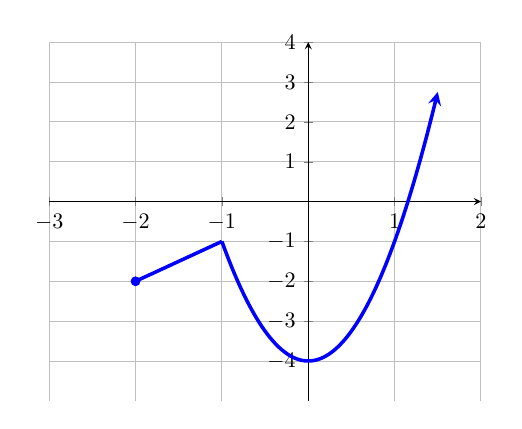
\begin{tikzpicture}[>=stealth, scale=0.8]
    \begin{axis}
    [axis lines = middle, grid,
    xmin = -3, xmax = 2, ymin = -5, ymax = 4,
    % xtick = {-2.5,-2,...,1.5}, 
    ytick = {-4,-3,...,4}
    ]
    \addplot[ultra thick, color=blue,samples=200, domain=-2:-1] {x};
    \addplot[->, ultra thick, color=blue, samples=200, domain=-1:1.5] {3*x^2-4};
    \addplot[color=blue, mark = *] coordinates {(-2,-2)};
    \end{axis}
    \end{tikzpicture}
\end{center}

\begin{multicols}{2}
\begin{enumerate}
\item Domain of $f$
\item Range of $f$
\item Relative Minimum
\item Relative Maximum
\item $f(1)$
\item $f(0)$
\item Increasing Interval(s)
\item Decreasing Interval(s)
\item Absolute Maximum
\item Absolute Minimum
\setcounter{Review}{\value{enumi}}
\end{enumerate}
\end{multicols}

Find each of the following given $f(x) = -2x^{3}+6x^{2}-5x+1$. Round to 3 decimal places and use interval notation when applicable.
\begin{multicols}{2}
\begin{enumerate}
\setcounter{enumi}{\value{Review}}
\item $f(7)$
\item $f(-2)$
\item Rel. Max
\item Rel. Min
\item Global Max
\item Global Min
\item Increasing Interval(s)
\item Decreasing Interval(s)
\setcounter{Review}{\value{enumi}}
\end{enumerate}
\end{multicols}

Use the graph of $f(x)$ to answer each.	\newline\\

\begin{center}
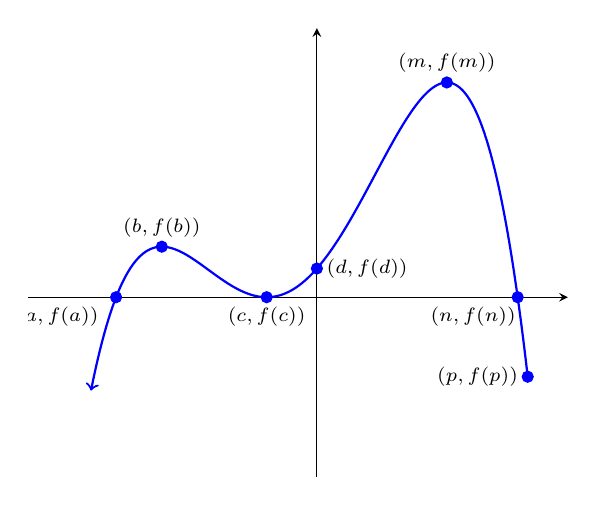
\begin{tikzpicture}[scale=1]
\begin{axis}[
axis lines = middle, xmin = -5.75, xmax = 5, ymin = -10, ymax = 15, ticks=none]
]
\addplot [<-,blue, thick, domain=-4.5:4.2, samples=200] {-0.1*(x+1)*(x+4)*(x+1)*(x-4)};
\addplot[blue, mark=*, only marks] coordinates {(-4,0) (-3.089,2.818) (-1,0) (0,1.6) (2.589,11.975) (4,0) (4.2,-4.434)};
\node at (axis cs: -4,0) [below left, xshift=-0.1cm] {\scriptsize$(a, f(a))$};
\node at (axis cs: -3.089,2.818) [above] {\scriptsize$(b, f(b))$};
\node at (axis cs: -1,0) [below] {\scriptsize$(c, f(c))$};
\node at (axis cs: 0,1.6) [right] {\scriptsize$(d, f(d))$};
\node at (axis cs: 2.589,11.975) [above] {\scriptsize$(m, f(m))$};
\node at (axis cs: 4,0) [below left, xshift=0.1cm] {\scriptsize$(n, f(n))$};
\node at (axis cs: 4.2,-4.434) [left] {\scriptsize$(p, f(p))$};
\end{axis}
\end{tikzpicture}
\end{center}

\begin{multicols}{2}
\begin{enumerate}
\setcounter{enumi}{\value{Review}}
\item Relative maxima of $f(x)$
\item Relative minima of $f(x)$
\item Absolute maxima of $f(x)$
\item Absolute minima of $f(x)$
\item Intervals where $f$ is increasing
\item Intervals where $f$ is decreasing
\item Zeros of $f$
\end{enumerate}
\end{multicols}

\newpage

\textsc{Properties of Functions Key} 

\section*{Maxima and Minima}

\begin{enumerate}
	\item Rel max @ $(0,5)$; No rel min
	\item Rel max @ $(2.158, 3.248)$; Rel min @ $(-1.158, -4.048)$
	\item Rel Max $(-1.366,10.848)$ and $(1,6)$; \quad Rel Min $(0.366,5.652)$
    \item Rel Max $(-1.716,11.598)$; \quad Rel Min $(1.132,-3.929)$
    \item Rel Max: $(1.095, 12.096)$; \quad Rel Min $(-0.761, -0.680)$
    \item Rel Max: $(1.366, 0.348)$; \quad
    Rel Min: $(-0.366, -4.848)$ and $(2,0)$
	\item About 2.16 hours
\end{enumerate}

\section*{Increasing, Decreasing, and Constant Intervals}

\begin{enumerate}
	\item Increasing: $(-\infty, 0)$ \quad Decreasing: $(0, \infty)$
	\item Increasing: $(-1.158, 2.158)$ \quad Decreasing: $(-\infty, -1.158) \cup (2.158, \infty)$
    \item Inc: $(-\infty,-2) \cup \left(\frac{2}{3},\infty\right)$ \quad Dec: $\left(-2, \frac{2}{3}\right)$
    \item Inc; $(-1,0) \cup (1, \infty)$ \quad Dec: $(-\infty, -1) \cup (0,1)$
    \item Inc: $(-1,\infty)$ \quad No intervals where it is decreasing
    \item Inc: $(-0.761, 1.095)$; \quad Dec: $(-\infty, -0.761) \cup (1.095, \infty)$
    \item Inc: $(-0.366,1.366) \cup (2, \infty)$; \quad
    Dec: $(-\infty, -0.366) \cup (1.366,2)$;
\end{enumerate}

\section*{Miscellaneous}

\begin{multicols}{2}
\begin{enumerate}
    \item $[-2, \infty)$
    \item $[-4, \infty)$
    \item $(0, -4)$
    \item $(-1,-1)$
    \item $-1$
    \item $-4)$
    \item $(-2, -1) \cup (0, \infty)$
    \item $(-1,0)$
    \item $(0,-4)$
    \item None
    \item $-426$
    \item 51
    \item (1.408, 0.272)
    \item $(0.592, \, -0.272)$
    \item None
    \item None
    \item $(0.592, \, 1.408)$
    \item $(-\infty, \, 0.592) \cup (1.408, \, \infty)$
	\item $(b, f(b))$ and $(m, f(m))$
	\item $(c, f(c))$
	\item $(m, f(m))$
	\item None
	\item $(-\infty, b) \cup (c, m)$
	\item $(b, c) \cup (m, p)$
	\item $x = a, \, x = c, \, x = n$
\end{enumerate}
\end{multicols}